\documentclass{standalone}

\begin{document}


\subsection[Compare dataset]{SNP classification}\label{rfbp:snp}

Few available applications of the rFBP algorithm to real data are amenable to two aspects: I) learning technique; II) algorithm implementation.
The first one is related to the intrinsic definition of the algorithm which is designed to reach a complete memorization of the training dataset; in the other Machine Learning processes we normally want to avoid this kind of results since it could bring to \emph{over-fitting} problems.
The second one is given by the binary values involved in each step of the algorithm which intrinsically limits the possible applications\footnote{
  The Neural Network weights can assume only binary values since they model up/down spins.
  Moreover also the input is required to be a spin configuration and thus binary.
  The common Machine Learning problems involve floating-point values as input pattern and it is not straightforward their conversion to binary values without loosing information.
}.

Classification problems which involve only binary quantities are quite small but the GWA is one of them.
In the GWA we have a series of genome data belonging to different classes as input.
A genome is the ensemble of genes of an organism and each gene is identified by a series of nucleotides with 4 possible values (G, guanine; C, cytosine; A, adenine; T, thymine).
The comparison between a reference (healthy) genome and an infected one highlights the biological mutation related to the underlying disease.
These mutations are the so-called SNPs (Single Nucleotide Polymorphisms).
Thus, we can identify a genome as a sequence of its mutation in relation to a reference one, i.e a sequence of two possible values given by the on/off of nucleotide mutation.

The COMPARE project aims to develop new methods to avoid the genetic disease transmission.
In this project plays a crucial role the \emph{Source Attribution}, i.e the classification of a given disease based on the list of its mutation.

We tested the rfBP on $210$ Salmonella enterica genome sequences, $4857450\,bp$ (base pairs) long, living inside animals.
Our early goal was to discriminate bacteria which lives in pigs (159 samples) against to all the others animals (51 samples).

\begin{figure}[htbp]
\centering
% \def\svgwidth{\textwidth}
% \input{./img/Sequences.pdf_tex}
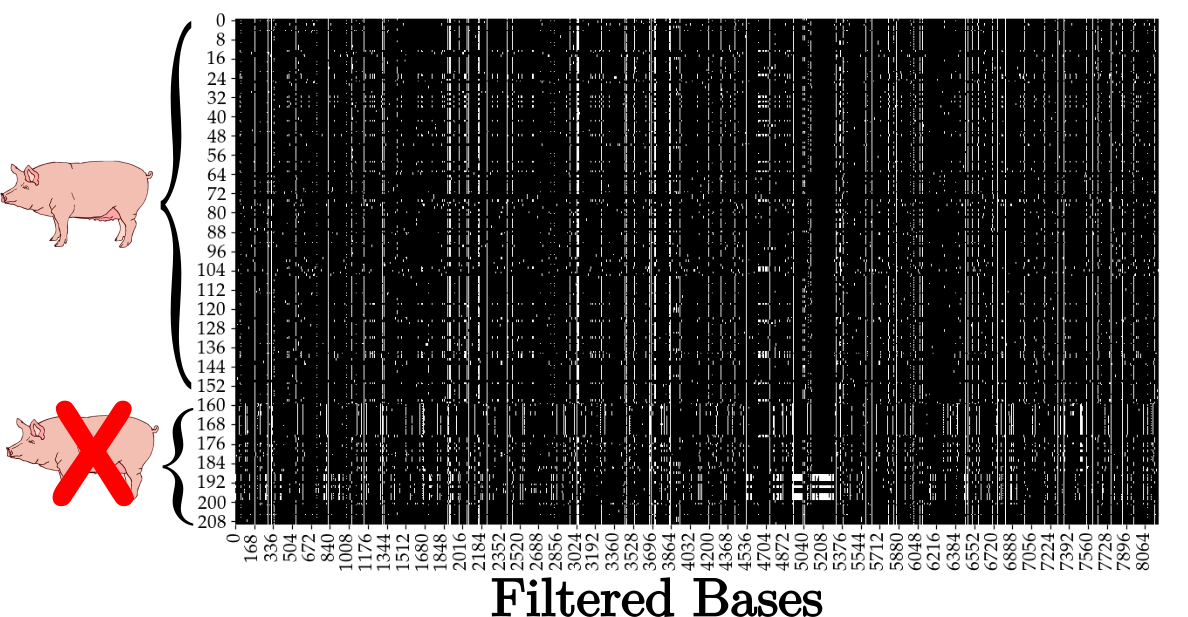
\includegraphics[width=0.85\textwidth]{Sequences.png}
\caption{SNP sequences of Salmonella enterica samples used in this work.
The x-axis shows the genome bases and the y-axis the corresponding sample (210 samples in total).
The black dots are related to a base without mutation (in relation to the genome reference), while the with dots are the mutation (SNPs) identified.
The first 159 rows contain the genome sequences related to pigs, i.e the sequences obtained by a pig which host the bacteria, and the following ones contain sequences of other animals.
Also with naked eyes we can see the differences between the two data types.
}
\label{fig:SNPsAle}
\end{figure}

First of all, we filtered our data removing from each genome a base if it showed a mutation in all the samples.
In this way we reduced the number of bases to $8189\,bp$.
A graphical representation of these samples is given in Fig.~\ref{fig:SNPsAle}.
The dataset was divided in training and test sets using a stratified cross-validation procedure to guarantee a proportional subdivision of the samples into the two classes.
The algorithm hyper-parameters were tuned on the training set in relation to the performances obtained using a internal stratified 10-fold cross-validation: in each fold the training was performed using a sequence of hyper-parameters and the performances evaluated on the corresponding test set; the hyper-parameters configuration which obtained the best performances on the full training set was chosen as best one.
We use our custom \emph{Scorer} library for the performance evaluation.
Considering the unbalanced sample quantities the Matthews Correlation Coefficient (MCC) was chosen as good score indicator for the evaluation.

\end{document}
